\documentclass[11pt]{article}
\usepackage{fancyhdr}
\usepackage{graphicx}
\usepackage{float}
\usepackage{amssymb,amsmath}
\usepackage{psfrag}
\usepackage{color}
\usepackage[colorlinks]{hyperref}
\usepackage[footnotesize,hang,bf]{caption}
\usepackage{subeqnarray}
% \usepackage{amsthm}
 \usepackage{enumitem}
 \graphicspath{{Figures/}}
% \usepackage{multicol}
 \usepackage{ marvosym }
 \usepackage{wasysym}
 \usepackage{tikz}
 \usepackage[capitalize]{cleveref}
\usepackage{ifthen,verbatim,color}
 \usetikzlibrary{patterns}

 \newcommand{\ds}{\displaystyle}
 \DeclareMathOperator{\sech}{sech}

%%%%%%%%%%%%%%%%%%%%%%%%%%%%%%%%%%%%%%%%%%%%%%%%%%%%%%%%%%%%%%%%%%%%%%%%%%%%%%%%%%

\def\term{Spring 2018}

\setlength{\oddsidemargin}{0 in}
\setlength{\evensidemargin}{0 in}
\setlength{\topmargin}{0.0 in}
\setlength{\textwidth}{6.45 in}
\setlength{\textheight}{8.5 in}
%\setlength{\headheight}{1 in}
\renewcommand{\baselinestretch}{0.95}

\pagestyle{fancy}
\rhead{ME 257/357\\ \term \\Mid-term Exam}
\lhead{}
\renewcommand{\headrulewidth}{0pt}

\makeatother
% Environment for problem solutions
\newboolean{showsolutions}
% Set showsolutions to 'true' or 'false'
\setboolean{showsolutions}{true}

\newenvironment{solution}
{
  \ifthenelse{\boolean{showsolutions}}
  {\color{blue}\par\medskip\underline{\textbf{Solution}}\par\medskip}
  {\expandafter\comment}
}
{
  \ifthenelse{\boolean{showsolutions}}
  {}
  {\expandafter\endcomment}
}

\begin{document}

\begin{center}
{\Large\bf ME 257/357 Gas Turbine Design: Mid-term\\
       Thursday, 5/24/2018, 10:30 - 11:50 am}
\end{center}

\hrule
\vspace{2mm}
%=======================================================================================================
\noindent Write your name on this handout and sign the honor code:

\vspace{6mm}
\noindent \textbf{Name}: \dotfill % \hfill\null
\vspace{2mm}

\noindent \textbf{Honor Code}: \emph{I have neither given nor received unauthorized aid on this examination, nor have I concealed any violations of the Honor Code.}

\vspace{6mm}
\noindent \textbf{Signiture}: \dotfill % \hfill\null 

\vspace{2mm}
\noindent This exam consists of two parts. Part 1 contains 10 short-answer problems (\emph{4 pts} each) and Part 2 consider a detailed analysis of a turbofan engine. You need to complete both parts for full credit. The exam is open-book/open-notes and no external resources are allowed. Plan on not taking more than 30 mins for Part 1. The total points is 100.

\vspace{2mm}
\hrule

%=======================================================================================================
\vspace{2mm}

\section*{\textbf{PART 1:} CONCEPTUAL QUESTIONS (40 pts)} % (fold)
\label{sec:_textbf_part_1_short_answers}
This part tests your conceptual understanding of the course-material. Provide a brief but clear explanation or sketch for each question. Provide answers to each question in the blue book.

\begin{itemize}
	\item[(1)] Write down the equation for the drag coefficient of a wing with \emph{finite span}. Identify each term in the equation. Draw the drag polar.
	
	\item[(2)] Write down the thrust required for a steady level flight. Sketch $T^*$ as a function of the dynamic pressure $q_\infty$. 
	
	\item[(3)] What is the Breguet range equation? Sketch qualitatively the endurance factor as a function of the Mach number. Show curves at three different altitudes and explain why you drew them in this way.
	
	\item[(4)] Write down the thrust equation for an air-breathing propulsion system. Explain what will change when applying the thrust equation to a rocket engine. Show the final equation.
	
	\item[(5)] What is a single crystal blade? Write down three advantages of using the single crystal technology for turbine blades.
	
	\item[(6)] Name three pollutants that are generated in the combustion process. Briefly explain how does each pollutant form and how to reduce it.
	
	\item[(7)] Schematically draw a RQL combustor. Identify the combustion processes in each zone. Write down an equation (in symbolic form) that allows you to compute the density of the gas in the dilution region. Clearly state all assumptions.
	
	\item[(8)] Define choke and stall in a compressor stage and explain their consequences.
	
	\item[(9)] Draw the compressor map qualitatively. Mark all important features on the graph.
	
	\item[(10)] Briefly explain why the isentropic efficiency of a compressor is typically smaller than that of a turbine.
	
\end{itemize}

% section _textbf_part_1_short_answers (end)

\newpage


\section*{\textbf{PART 2:} ENGINE ANALYSIS (60 pts)} % (fold)
\label{sec:_textbf_part_2_engine_analysis}
\noindent {In this part of the exam you are asked to provide a detailed analysis of a turbofan engine. Clearly write down your derivation steps and mark the final results.}

\section*{Problem description} % (fold)
\label{sub:low_order_design_of_a_turbofan_engine}
\noindent In this problem, you will analyze a GE 90 turbofan engine (as shown in~\cref{fig:engine}) with efficiencies of each component listed in~\cref{tab:eff}. The free stream Mach number is $M_0 = 0.85$, temperature is $T_0 = 220$ K, and pressure is $P_0 = 24$ kPa. The core mass flow rate of air is $\dot{m}_{a,c} = 3.0$ kg/s, the bypass ratio is $2.9$, the fan pressure ratio is $2.0$.

\begin{figure}[!htb!]
	\centering
	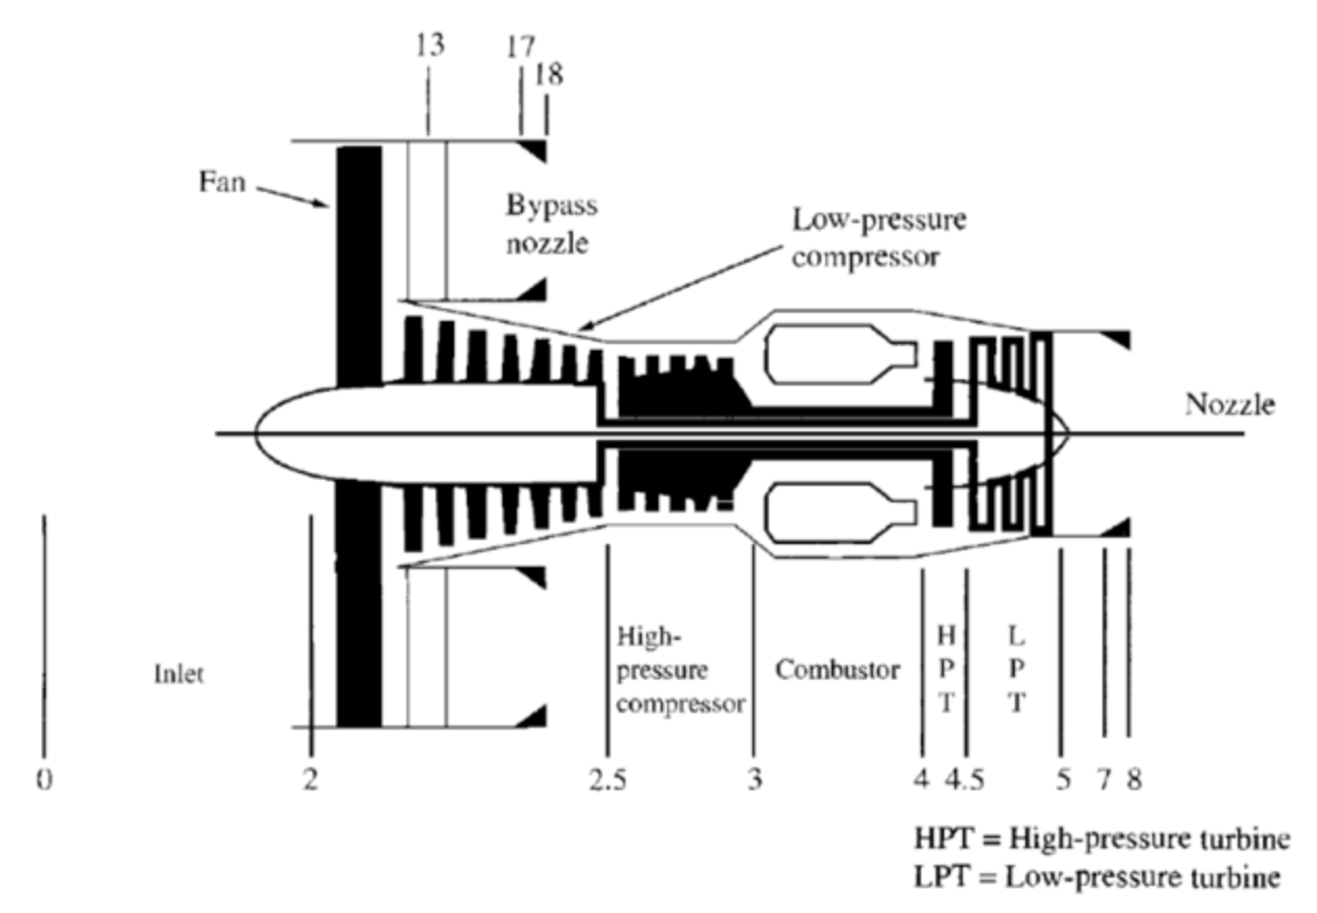
\includegraphics[width=0.6\textwidth]{engine.pdf}
    \caption{Schematic of the GE90 engine with station numbering.}
	\label{fig:engine}
\end{figure}

\begin{table}[ht!]
	\caption{Turbofan component efficiencies.}
	\label{tab:eff}
	\centering
	\begin{tabular}{ | c | c |} 
			\hline
 		   	Component & $\eta_\text{adiabatic}$ \\\hline 
			\hline
			Diffuser & $95\%$ \\ 
			Fan & $92\%$ \\
			Compressor & $87\%$ \\
			Combustor & $100\%$ \\
			Turbine (LPT \& HPT) & $91\%$ \\
			Core/Fan nozzle & $98\%$ \\
			\hline
	\end{tabular}
\end{table}

\newpage

\section{Compressor analysis (15 pts)}
\begin{enumerate}
		\item[(a)](5 pts) For a single compressor stage (consider the first stage after the inlet guide vane) shown in~\cref{fig:compressor}, complete the velocity triangle across the rotor at the pitchline $r_m$. Assume the following quantities as known: the inlet velocity $U_{c1}$, the angle of attack of the flow after the inlet guide vane $\alpha_{c1}$, the angular velocity of the compressor $\Omega$, the relative angle at the rotor leading edge $\beta_{c1}$, and the relative angle at the rotor trailing edge $\beta_{c2}$. Express $U_{c1,\theta}$, $U_{c2,\theta}$, and $\alpha_{c2}$ using the known quantities.
		
		\begin{figure}[ht]
			\centering
			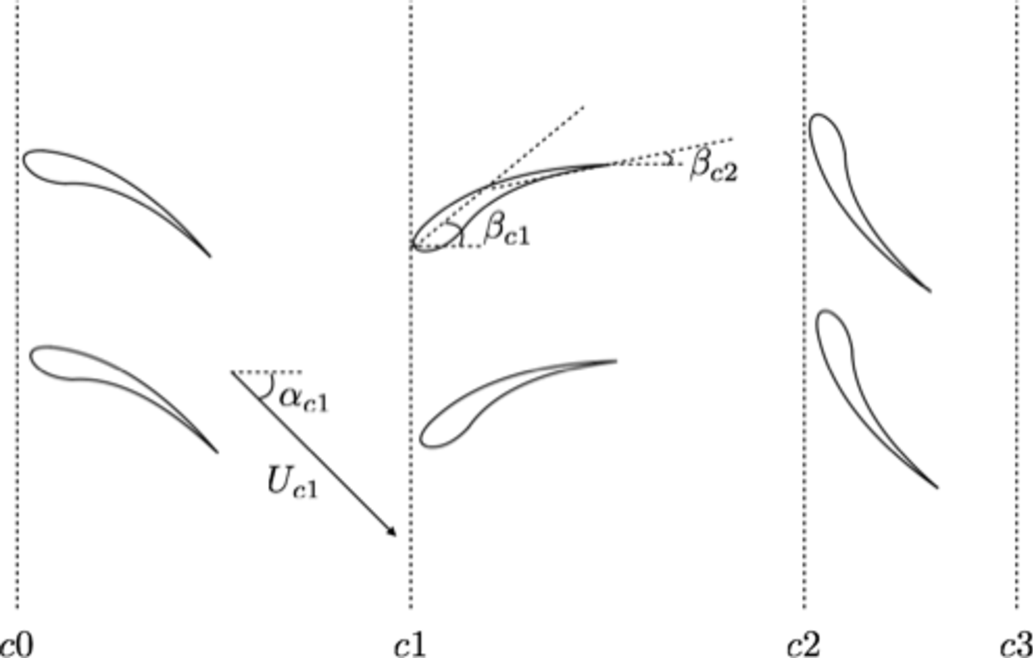
\includegraphics[width=0.6\textwidth]{compressor.pdf}
		    \caption{Schematic of the the first compressor stage with station numbering.}
			\label{fig:compressor}
		\end{figure}
		
		\begin{solution}
			\begin{figure}[ht]
				\centering
				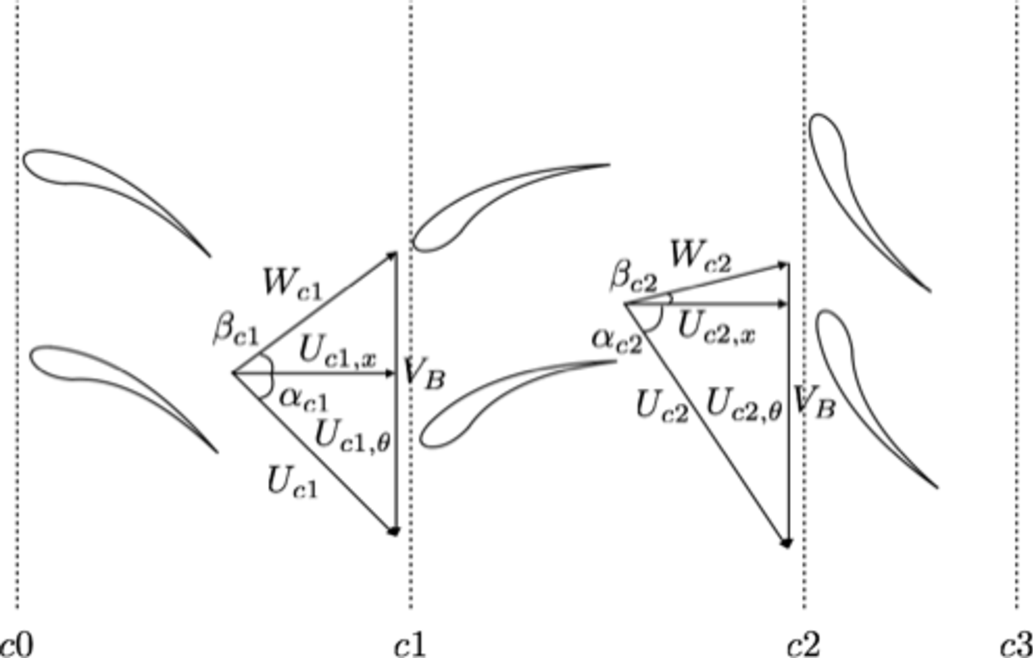
\includegraphics[width=0.6\textwidth]{compressor_soln.pdf}
			    \caption{Schematic of the the first compressor stage with station numbering.}
				\label{fig:compressor_soln}
			\end{figure}
		\end{solution}
		
		\item[(b)] (5 pts) What is the work consumed by this compressor stage? Assuming the inlet velocity $U_{c1} = 150$ m/s, the angular velocity is $\Omega = 24000$ rpm, the vortex design follows the \emph{constant reaction} specification, the angle of attack at the hub and tip are $\alpha_{c1,\text{tip}} = 30^\circ$ and $\alpha_{c1,\text{tip}} = 23.8^\circ$, the radius at the hub and the tip are $r_\text{hub} = 0.9$ m and $r_\text{tip} = 1.0$ m, respectively.
		
		\begin{solution}
			From the vortex design of the \emph{constant reaction} specification, i.e.
			\begin{align}
				rU_{c1,\theta} &= -b + a r^2, \\
				rU_{c2,\theta} &= b + a r^2. \label{eq:U_theta2}
			\end{align}
			Substituting $r_\text{hub}$, $\alpha_{c1,\text{hub}}$ and $r_\text{tip}$, $\alpha_{c1,\text{tip}}$ into~\cref{eq:U_theta2}, coefficients $a$ and $b$ are obtained as:
			 \begin{align}
				a &= \frac{\sin \alpha_{c1,\text{tip}} / r_\text{tip} - \sin \alpha_{c1, \text{hub}} / r_\text{hub}}{1/ r_{c1, \text{tip}}^2 - 1 / r_{c1,\text{hub}}^2} U_{c1} = 145.8, \\
				b &= \frac{r_\text{tip} \sin \alpha_{c1,\text{tip}} - r_\text{hub} \sin \alpha_{c1,\text{hub}}}{r_{\text{tip}}^2 - r_{\text{hub}}^2} U_{c1} = -0.245.
			 \end{align}
			 Therefore the work across this stage is:
			 \begin{align}
			 	h_{0c3} - h_{0c1} &= V_B \Delta U_{c, \theta} \\
								  &= (r \Omega)(2 a /r) \\
								  &= 2 a \Omega = 7\text{ MJ}.
			 \end{align}
		\end{solution}
		
		\item[(c)] (5 pts) What is pressure ratio across this stage? Assuming there are three identical stages, what is the overall pressure ratio provided by the compressor?
		
		\begin{solution}
			The pressure ratio across this single stage is:
			\begin{align}
				\frac{p_{0, c3}}{p_{0, c1}} &= \frac{1}{\pi \left( r_{\text{tip}}^2 - r_{\text{hub}}^2\right)}\int_{r_\text{hub}}^{r_\text{tip}} 2 \pi r \left(1 + \eta_\text{st} \frac{V_B \Delta U_\theta}{Cp T_{0, c1}}\right)^{\frac{\gamma}{\gamma - 1}} dr \\
				&= \left(1 + \eta_\text{st} \frac{V_B \Delta U_\theta}{Cp T_{0, c1}}\right)^{\frac{\gamma}{\gamma - 1}} \\
				&= 2.71.
			\end{align}
			Assuming the stages are identical, the overall compression ratio is:
			\begin{equation}
				\frac{p_{03}}{p_{02.5}} = \left(\frac{p_{0, c3}}{p_{0, c1}}\right)^3 = 20.
			\end{equation}
		\end{solution}
		
		\item[(d)] \emph{bonus (5 pts)}: what is the degree of reaction for this compressor stage?
	\end{enumerate}


\section{Combustor analysis (15 pts)}
	\begin{itemize}
		\item[(a)] (5 pts) n-Hexadecane (C$_{16}$H$_{34}$) is used in the current engine. Write down the reaction equation for the oxidation with air at  stoichiometric conditions.  Assuming the fuel-to-air ratio is $f=0.0043$, what is the equivalence ratio in this combustor?
		
		\begin{solution}
			The equivalence ratio is $\phi = f/f_\text{st} = 0.064$.
		\end{solution}
		
		\item[(b)] (5 pts) What is the lower heating value of the reaction for the given fuel-to-air ratio?
		
		\begin{solution}
			The lower heating value is $LHV = 153.4$ kcal/mol.
		\end{solution}
		
		\item[(c)] (5 pts) Compute the adiabatic flame temperature assuming calorically perfect gas with $\gamma = 1.4$. Use this temperature as combustor exit temperature $T_{04}$.
		
		\begin{solution}
			The adiabatic flame temperature is $T04 = 1600.3$ K.
		\end{solution}
		
	\end{itemize}

\newpage
\section{Brayton Cycle Analysis (30 pts)}
\begin{itemize}
	\item[(a)] (20 pts) Perform the Brayton cycle analysis to the engine using the $T$-$s$ diagram shown in~\cref{fig:Ts}. Ignore the low-pressure compressor, i.e. assume that the low-pressure turbine drives the fan only. Assume the pressure at the core nozzle exit is the same as the free stream pressure. Complete the $T$-$s$ diagram with the numbers obtained from the cycle analysis. Mark each station clearly and draw addition constant pressure lines if necessary. Station 0 has been marked for you. 
	
	\begin{figure}[ht]
		\centering
		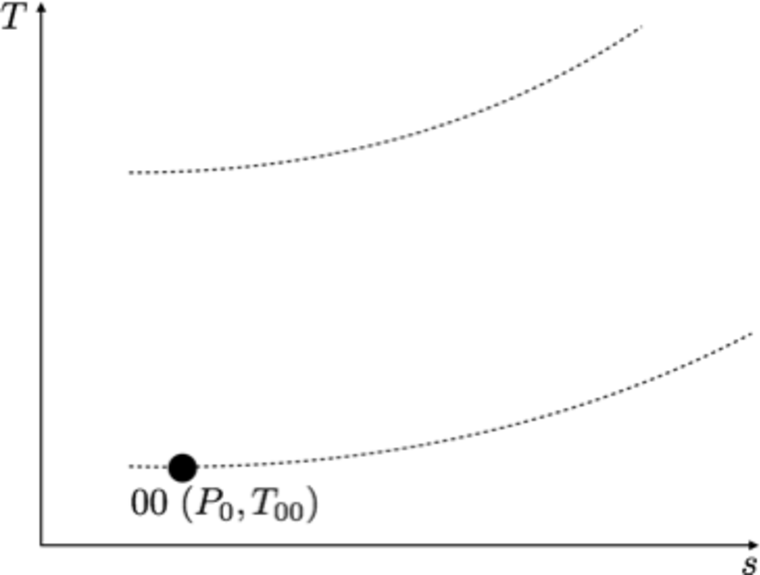
\includegraphics[width=0.6\textwidth]{Ts_diagram.pdf}
	    \caption{T-s diagram of the Brayton cycle analysis to the GE90 engine.}
		\label{fig:Ts}
	\end{figure}
	
	\begin{solution}
		Note that the stagnation temperature is:
		\begin{equation}
			\frac{T_{0}}{T} = 1 + \left(\frac{\gamma - 1}{2}\right)M^2.
		\end{equation}
		The isentropic state relationship is:
		\begin{equation}
			\frac{p_{0}}{p} = \left(\frac{T_{0}}{T}\right)^{\frac{\gamma}{\gamma - 1}}.
		\end{equation}
		For real engines with none unity efficiencies, it is required to relate the real stagnation states with the isentropic states. Here, it is assumed that the gas is Calorically perfect, i.e. $C_p$ is constant. It is also assumed that $p_0/p_{0s} = 1$. For components with pressure increases, e.g. diffusor, fan, and compressor, the efficiency from station $a$ to $b$:
		\begin{align}
			\eta &= \frac{h_{0bs} - h_{0a}}{h_{0b} - h_{0a}} \\
				 &= \frac{T_{0bs} - T_{0a}}{T_{0b} - T_{0a}} \\
				 &= \frac{T_{0bs}/T_{0a} -1}{T_{0b}/T_{0a} - 1}.
		\end{align}
		With this,
		\begin{align}
			T_{0b}/T_{0a} &= 1 + \frac{1}{\eta}\left(\frac{T_{0bs}}{T_{0a}} -1\right), \\
			T_{0bs}/T_{0a} &= 1 + \eta\left(\frac{T_{0b}}{T_{0a}} -1\right).
		\end{align}
		If the pressure ratio $p_{0b}/p_{0a}$ is known, the temperature ratio is found as:
		\begin{align}
			T_{0b}/T_{0a} &= 1 + \frac{1}{\eta}\left(\frac{T_{0bs}}{T_{0a}} -1\right), \\
						  &= 1 + \frac{1}{\eta}\left[\left(\frac{p_{0b}}{p_{0a}}\right)^{\frac{\gamma - 1}{\gamma}} -1\right].
		\end{align}
		If the temperature ratio $T_{0b}/T_{0a}$ is known, the pressure ratio is found as:
		\begin{align}
			p_{0b}/p_{0a} &= \left(T_{0bs}/T_{0a}\right)^{\frac{\gamma}{\gamma - 1}} \\
						  &= \left[1 + \eta\left(\frac{T_{0b}}{T_{0a}} -1\right) \right]^{\frac{\gamma}{\gamma - 1}}.
		\end{align}
		For components with pressure decreases, e.g. turbine and nozzle, the efficiency from station $a$ to $b$ is defined as:
		\begin{align}
			\eta &= \frac{h_{0a} - h_{0b}}{h_{0a} - h_{0bs}} \\
				 &= \frac{T_{0a} - T_{0b}}{T_{0a} - T_{0bs}} \\
				 &= \frac{1 - T_{0b}/T_{0a}}{1 - T_{0bs}/T_{0a}}.
		\end{align}
		With this,
		\begin{align}
			T_{0b}/T_{0a} &= 1 - \eta\left(1 - T_{0bs}/T_{0a}\right), \\
			T_{0bs}/T_{0a} &= 1 - \frac{1}{\eta}\left(1 - \frac{T_{0b}}{T_{0a}}\right).
		\end{align}
		If the pressure ratio $p_{0b}/p_{0a}$ is known, the temperature ratio is found as:
		\begin{align}
			T_{0b}/T_{0a} &= 1 - \eta\left(1 - T_{0bs}/T_{0a}\right), \\
						  &= 1 - \eta\left[1 - \left(p_{0b}/p_{0a}\right)^{\frac{\gamma - 1}{\gamma}}\right].
		\end{align}
		If the temperature ratio $T_{0b}/T_{0a}$ is known, the pressure ratio is found as:
		\begin{align}
			p_{0b}/p_{0a} &= \left(T_{0bs}/T_{0a}\right)^{\frac{\gamma}{\gamma - 1}} \\
					      &= \left[1 - \frac{1}{\eta}\left(1 - \frac{T_{0b}}{T_{0a}}\right)\right]^{\frac{\gamma}{\gamma - 1}}.
		\end{align}
		
		With these relationships, the Brayton cycle analysis for the turbofan engine is performed as follows.
		\begin{itemize}
			\item \emph{Diffuser ($0\rightarrow 2$)}
			
				Stagnation temperature at station 2:
				\begin{equation}
					\frac{T_{02}}{T_{0}} = 1 + \left(\frac{\gamma - 1}{2}\right)M^2.
				\end{equation}
				The pressure ratio is hence:
				\begin{equation}
					\frac{p_{02}}{p_{0}} = \left[1 + \eta\left(\frac{T_{02}}{T_{0}} -1\right) \right]^{\frac{\gamma}{\gamma - 1}}.
				\end{equation}
				
			\item \emph{Fan ($2\rightarrow 2.5/13$)}
				
				Given pressure ratio across the fan $p_{02.5}/p_{02}$ (note that $p_{02.5} = p_{013}$), the temperature ratio is:
				\begin{equation}
					\frac{T_{02.5}}{T_{02}} = 1 + \frac{1}{\eta}\left[\left(\frac{p_{02.5}}{p_{02}}\right)^{\frac{\gamma - 1}{\gamma}} -1\right].
				\end{equation}
			
			\item \emph{High Pressure Compressor ($2.5\rightarrow 3$)}
			
				The pressure ratio is obtained from previous problem as $p_{03}/p_{02.5}$, the temperature ratio is:
				\begin{equation}
					\frac{T_{03}}{T_{02.5}} = 1 + \frac{1}{\eta}\left[\left(\frac{p_{03}}{p_{02.5}}\right)^{\frac{\gamma - 1}{\gamma}} -1\right].
				\end{equation}
				
			\item \emph{Combustor ($3\rightarrow 4$)}
			
				The stagnation temperature at station 4 is obtained from previous problem as $T_{04} = T_{ad}$. With the assumption that the efficiency is 1 for the combustor, $p_{04}/p_{03} = 1$.
				
			\item \emph{High-Pressure Turbine ($4\rightarrow 4.5$)}
			
				From work balance between the high-pressure turbine and the high-pressure compressor:
				\begin{equation}
					(\dot{m}_{a,c} + \dot{m}_f)(T_{04} - T_{04.5}) = \dot{m}_{a,c}(T_{03} - T_{02.5}),
				\end{equation}
				the temperature ratio is obtained as:
				\begin{equation}
					\frac{T_{04.5}}{T_{04}} = 1 - \frac{1}{1 + f}\frac{T_{03} - T_{02.5}}{T_{04}}.
				\end{equation}
				The pressure ratio is then:
				\begin{equation}
					p_{04.5}/p_{04} = \left[1 - \frac{1}{\eta}\left(1 - \frac{T_{05}}{T_{04}}\right)\right]^{\frac{\gamma}{\gamma - 1}}.
				\end{equation}
				
			\item \emph{Low-Pressure Turbine ($4.5\rightarrow 5$)}
				
				From work balance between the low-pressure turbine and the fan:
				\begin{equation}
					(\dot{m}_{a,c} + \dot{m}_f)(T_{04.5} - T_{05}) = \beta\dot{m}_{a,c}(T_{02.5} - T_{02}),
				\end{equation}
				the temperature ratio is obtained as:
				\begin{equation}
					\frac{T_{05}}{T_{04.5}} = 1 - \frac{\beta}{1 + f}\frac{T_{02.5} - T_{02}}{T_{04.5}}.
				\end{equation}
				The pressure ratio is then:
				\begin{equation}
					p_{05}/p_{04.5} = \left[1 - \frac{1}{\eta}\left(1 - \frac{T_{05}}{T_{04.5}}\right)\right]^{\frac{\gamma}{\gamma - 1}}.
				\end{equation}
			
			\item \emph{Core Nozzle ($5\rightarrow 8$)}
			
				Note that $p_{08}/p_{05} = p_{00}/p_{05}$ is known, the temperature ratio is found as:
				\begin{equation}
					T_{08}/T_{05} = 1 - \eta\left[1 - \left(p_{08}/p_{05}\right)^{\frac{\gamma - 1}{\gamma}}\right].
				\end{equation}
			
			\item \emph{Fan/Bypass Nozzle ($13\rightarrow 18$)}
			
				Note that $p_{018}/p_{02} = p_{00}/p_{02}$ is known, the temperature ratio is found as:
				\begin{equation}
					T_{018}/T_{02} = 1 - \eta\left[1 - \left(p_{018}/p_{02}\right)^{\frac{\gamma - 1}{\gamma}}\right].
				\end{equation}
			
		\end{itemize}
	\end{solution}
	
	\item[(b)] (10 pts) Compute the following engine performance quantities:
	\begin{itemize}
		\item[(i)] (5 pts) What is the thrust generated by the engine? What is the TSFC?
		
		\begin{solution}
			The exit velocity of the fan and core nozzle are:
			\begin{align}
				U_{1e} &= \sqrt{2 \eta_f c_p T_{013}\left[ 1 - \left( \frac{p_0}{p_{013}}\right)^{\frac{\gamma - 1}{\gamma}}\right]}, \\
				U_{e} &= \sqrt{2 \eta_n c_p T_{05}\left[ 1 - \left( \frac{p_0}{p_{05}}\right)^{\frac{\gamma - 1}{\gamma}}\right]}.
			\end{align}
			The thrust generated by the engine is:
			\begin{equation}
				T = \dot{m}_{a,c}\left[(1 + f)U_e + \beta U_{1e} - (1 + \beta)U_0 \right].
			\end{equation}
			The thrust specific fuel consumption is:
			\begin{equation}
				TSFC = \frac{f}{(1 + f)U_e + \beta U_{1e} - (1 + \beta)U_0 }.
			\end{equation}
			
		\end{solution}
		
		\item[(ii)] (5 pts) What is the propulsive efficiency of the engine?.
		
		\begin{solution}
			The propulsive efficiency is:
			\begin{align}
				\eta_p &= \frac{\dot{m}_{a,c} U_0\left[ (1 + f)U_e + \beta U_{1e} - (1 + \beta)U_0\right]}{\frac{1}{2}\dot{m}_{a,c}\left[ (1 + f)U_e^2 + \beta U_{1e}^2 - (1 + \beta)U_0^2\right]} \\
					   &= \frac{2 U_0\left[ (1 + f)U_e + \beta U_{1e} - (1 + \beta)U_0\right]}{\left[ (1 + f)U_e^2 + \beta U_{1e}^2 - (1 + \beta)U_0^2\right]}.
			\end{align}
		\end{solution}
		
	\end{itemize}
		
\end{itemize}

% subsection low_order_design_of_a_turbofan_engine (end)

% section _textbf_part_2_detailed_analysis (end)

%=======================================================================================================
\end{document}
